% This file was created with matplot2tikz v0.4.0.
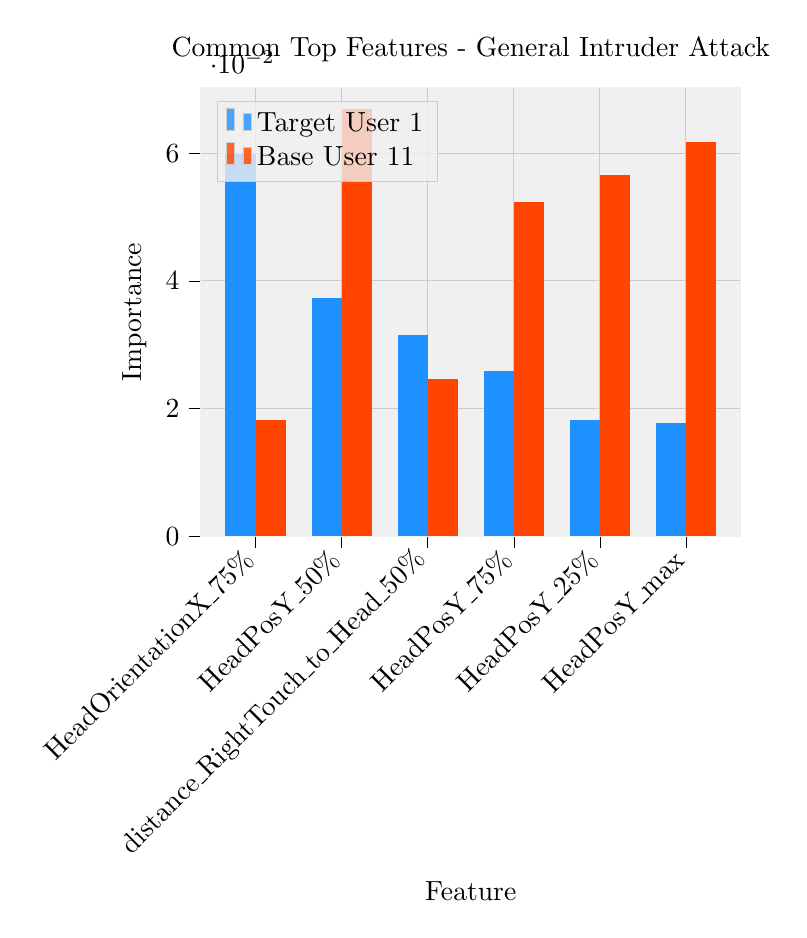
\begin{tikzpicture}

\definecolor{dodgerblue}{RGB}{30,144,255}
\definecolor{lightgray203}{RGB}{203,203,203}
\definecolor{lightgray204}{RGB}{204,204,204}
\definecolor{orangered}{RGB}{255,69,0}
\definecolor{whitesmoke240}{RGB}{240,240,240}

\begin{axis}[
axis background/.style={fill=whitesmoke240},
axis line style={whitesmoke240},
legend cell align={left},
legend style={
  fill opacity=0.8,
  draw opacity=1,
  text opacity=1,
  at={(0.03,0.97)},
  anchor=north west,
  draw=lightgray204,
  fill=whitesmoke240
},
tick align=outside,
tick pos=left,
title={Common Top Features - General Intruder Attack},
x grid style={lightgray203},
xlabel={Feature},
xmajorgrids,
xmin=-0.635, xmax=5.635,
xtick style={color=black},
xtick={0,1,2,3,4,5},
xticklabel style={rotate=45.0,anchor=east},
xticklabels={
  HeadOrientationX\_75\%,
  HeadPosY\_50\%,
  distance\_RightTouch\_to\_Head\_50\%,
  HeadPosY\_75\%,
  HeadPosY\_25\%,
  HeadPosY\_max
},
y grid style={lightgray203},
ylabel={Importance},
ymajorgrids,
ymin=0, ymax=0.070212958612367,
ytick style={color=black}
]
\draw[draw=none,fill=dodgerblue,very thin] (axis cs:-0.35,0) rectangle (axis cs:0,0.0599335978791356);
\addlegendimage{ybar,ybar legend,draw=none,fill=dodgerblue,very thin}
\addlegendentry{Target User 1}

\draw[draw=none,fill=dodgerblue,very thin] (axis cs:0.65,0) rectangle (axis cs:1,0.0372914184386497);
\draw[draw=none,fill=dodgerblue,very thin] (axis cs:1.65,0) rectangle (axis cs:2,0.0315592352680531);
\draw[draw=none,fill=dodgerblue,very thin] (axis cs:2.65,0) rectangle (axis cs:3,0.0258270556252948);
\draw[draw=none,fill=dodgerblue,very thin] (axis cs:3.65,0) rectangle (axis cs:4,0.018227246382557);
\draw[draw=none,fill=dodgerblue,very thin] (axis cs:4.65,0) rectangle (axis cs:5,0.0176766981287157);
\draw[draw=none,fill=orangered,very thin] (axis cs:2.77555756156289e-17,0) rectangle (axis cs:0.35,0.0182704498452303);
\addlegendimage{ybar,ybar legend,draw=none,fill=orangered,very thin}
\addlegendentry{Base User 11}

\draw[draw=none,fill=orangered,very thin] (axis cs:1,0) rectangle (axis cs:1.35,0.0668694843927305);
\draw[draw=none,fill=orangered,very thin] (axis cs:2,0) rectangle (axis cs:2.35,0.024658428536827);
\draw[draw=none,fill=orangered,very thin] (axis cs:3,0) rectangle (axis cs:3.35,0.0524051826548277);
\draw[draw=none,fill=orangered,very thin] (axis cs:4,0) rectangle (axis cs:4.35,0.0566175210214603);
\draw[draw=none,fill=orangered,very thin] (axis cs:5,0) rectangle (axis cs:5.35,0.0617358190739542);
\end{axis}

\end{tikzpicture}
